\chapter{Metodologia}\label{cap:metodologia}


Este trabalho de conclusão de concurso será dividido em quatro fases:
Pesquisa, Desenvolvimento, Testes e Monografia.

Durante a pesquisa científica, os artigos referenciados serão explorados com
maior atenção e será buscado entender os detalhes que implicam
na criação da técnica proposta. Em especial, dois artigos terão maior
atenção inicialmente: \textit{Network Unfolding Map By Vertex-Edge
  Dynamics Modeling} \cite{VerriNetworkUnfoldingMap2018} e
\textit{Image Segmentation Methods Based on Superpixel Techniques A
  Survey} \cite{SuperpixelSurvey2020}. O primeiro contém a definição
da técnica LCU, uma dinâmica coletiva sobre redes complexas, o
componente de aprendizagem principal do algoritmo; o segundo será
usado como uma pré-segmentação inicial antes de partir pra construção
da rede complexa. Na figura \ref{fig:fluxograma-algoritmo} é demonstrada uma
visão macro do algoritmo.

\begin{figure}[!h]
        \captionsetup{width=8cm}
		\Caption{\label{fig:fluxograma-algoritmo}
          Algoritmo de segmentação semi-supervisionada de imagens}
		\centering
		\UFCfig{}{
			\fbox{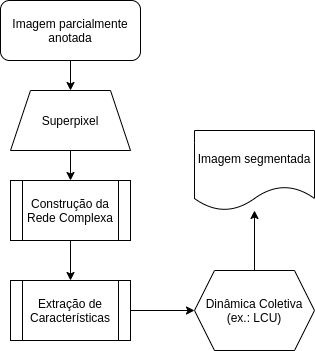
\includegraphics[width=8cm]{figuras/algorithm}}
		}{
			\Fonte{Autoral}
		}
\end{figure}


O desenvolvimento se concentrará na integração das técnicas
mencionadas acima como uma nova técnica de segmentação de imagens
semi-supervisionada, portanto, serão detalhadadas todas as
etapas necessárias pra construção e aplicação do novo algoritmo de
segmentação. Por exemplo, a construção da rede complexa assumirá
que cada superpixel será um vértice do grafo com seus vizinhos baseado
na topologia da imagem, a etapa de extração de características
ocorrerá em cada superpixel e a dinâmica coletiva considerará a
anotação parcial da imagem. No fim do algoritmo, os segmentos da
imagem serão subgrafos dessa rede complexa.

Adicionalmente, a implementação do algoritmo nesse trabalho será
construída de maneira \textit{Open Source} como uma ferramenta de
simulação de segmenteção, usando a biblioteca \gls{OpenCV} para que possa
ser testado o algoritmo de segmentação de imagens recebendo pontos
aleatórios de marcação do usuário. Isto simulará o caso de um
especialista analisando uma imagem médica, por exemplo.


Na fase de testes, a avaliação dos resultados considerará os
principais \textit{datasets} conhecidos para segmentação de imagens,
como o \textit{The Berkeley Segmentation Dataset and Benchmark}
\cite{MartinFTM01}.

Na fase de monografia serão consolidados todos os resultados em um
trabalho acadêmico nas normas da \gls{ABNT}.

O cronograma das atividades de pesquisa é apresentado a seguir.

\begin{table}[h]
\begin{tabular}{l|l|l|l|l|l|l|}
\cline{2-7}
                                          & Abril                                         & Maio                                            & Junho                                           & Julho                                           & Agosto                                          & Setembro                                        \\ \hline
\multicolumn{1}{|l|}{Pesquisa científica} & \multicolumn{1}{c|}{\cellcolor[HTML]{000000}} & \cellcolor[HTML]{000000}{\color[HTML]{000000} } & \cellcolor[HTML]{000000}{\color[HTML]{000000} } &                                                 &                                                 &                                                 \\ \hline
\multicolumn{1}{|l|}{Desenvolvimento}     &                                               &                                                 & \cellcolor[HTML]{000000}{\color[HTML]{000000} } & \cellcolor[HTML]{000000}{\color[HTML]{000000} } &                                                 &                                                 \\ \hline
\multicolumn{1}{|l|}{Testes}              &                                               &                                                 &                                                 & \cellcolor[HTML]{000000}{\color[HTML]{000000} } & \cellcolor[HTML]{000000}{\color[HTML]{000000} } &                                                 \\ \hline
\multicolumn{1}{|l|}{Monografia}          &                                               &                                                 &                                                 &                                                 & \cellcolor[HTML]{000000}{\color[HTML]{000000} } & \cellcolor[HTML]{000000}{\color[HTML]{000000} } \\ \hline
\end{tabular}
\end{table}
